\newcommand{\IbResposta}{Velocidade ótima \textbf{constante de \SI{20,7}{km/h}}, com partida às 17h45 (janela de 8\,h até 01h45); a viagem de \SI{7000}{km} termina em \textbf{248,8 dias} (\SI{28,1}{km/dia} em média) com reservas de 10\,\% na tração e 20\,\% nos serviços, ou 250,8 dias com reservas de 20/30\,\%.}
\newcommand{\IbResumo}{20,7 km/h constantes; 248,8 dias (26 km/dia em regime)}
\newcommand{\IbTexto}{%
A viagem parte com as duas baterias cheias (\SI{112,4}{kWh}) e só recebe energia solar. Nos primeiros 4 dias a bateria de tração desce até a reserva e o veículo percorre \SI{567}{km}; daí em diante cada dia roda o que o sol repôs, \SI{26,3}{km} em cerca de \SI{1,3}{h} de condução, bem abaixo do limite de 8\,h. Ao longo da viagem, os painéis geram \SI{3586}{kWh}: \SI{1279}{kWh} chegam à tração e \SI{1798}{kWh} abastecem a habitação (\SI{7,23}{kWh/dia}). A tração consome \SI{1366}{kWh} (\SI{0,195}{kWh/km}), em \SI{338}{h} de condução.

Como a energia solar diária é fixa, o tempo total é dominado pelos dias de espera para acumular energia, e não pelas horas ao volante. O tempo mínimo corresponde, portanto, à velocidade que minimiza o consumo por quilômetro, o mesmo $v^{*}$ do item 27; rodar mais rápido gasta mais energia por quilômetro e exige mais dias parados. Partir no fim da tarde deixa todo o período de sol com o veículo parado e os portáteis abertos.

O ótimo foi obtido em duas etapas: varredura de \num{2784} combinações (\SIrange{12}{40}{km/h} a cada \SI{1}{km/h}, partida a cada \SI{0,5}{h}, duas reservas) com passo de \SI{5}{min}, e refino de \num{294} casos (passo de \SI{0,1}{km/h} e \SI{0,25}{h}) com passo de \SI{1}{min}; o líder não está na borda da grade. Entre passos de 5 e \SI{1}{min} o tempo de viagem muda menos de \SI{0,03}{dias}.
\begin{figure}[H]\centering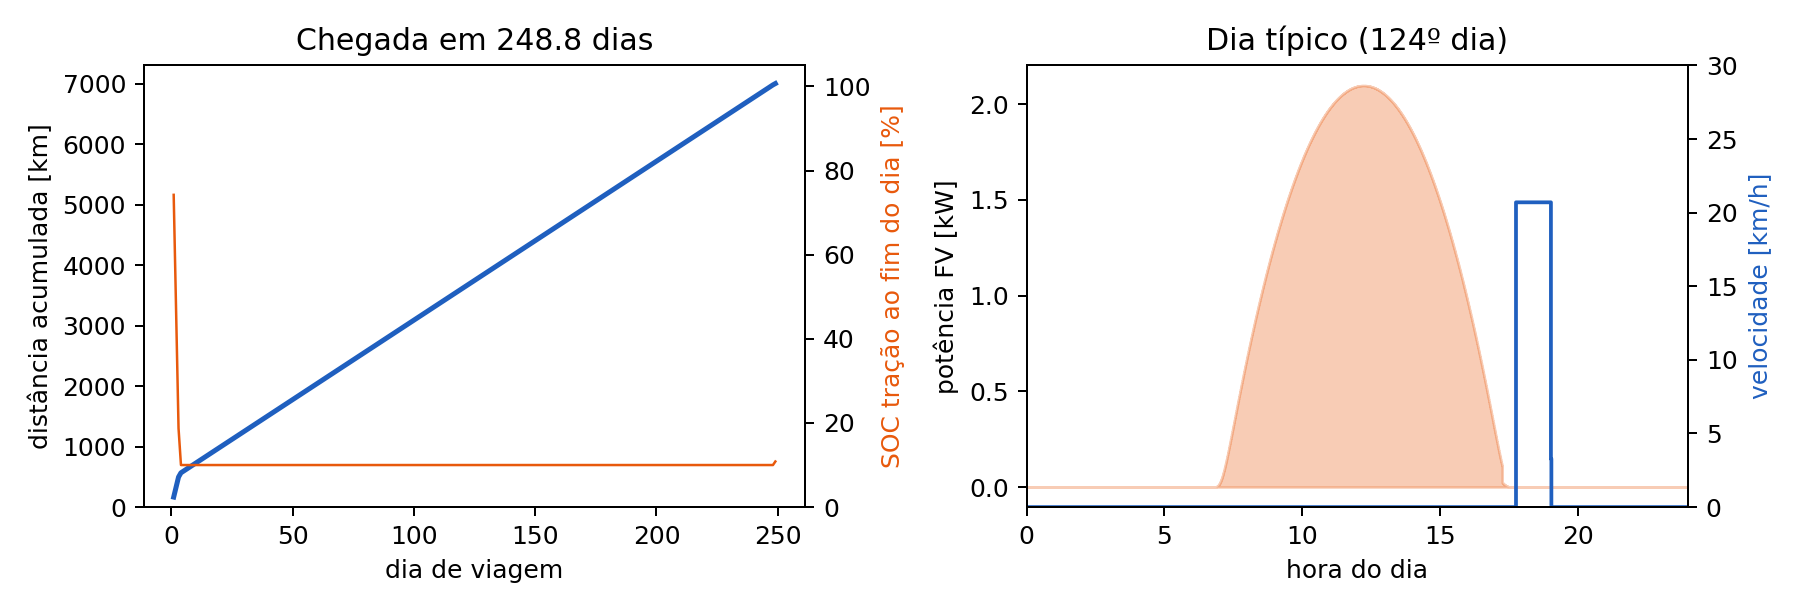
\includegraphics[width=\linewidth]{i29_missao.png}
\caption{Item 29 — distância acumulada e SOC da tração ao longo da viagem, e um dia típico.}\end{figure}}
